\documentclass[tikz, border=8pt]{standalone}
\usepackage{tikz}
\usetikzlibrary{arrows.meta, decorations.pathreplacing, calc}

\begin{document}
    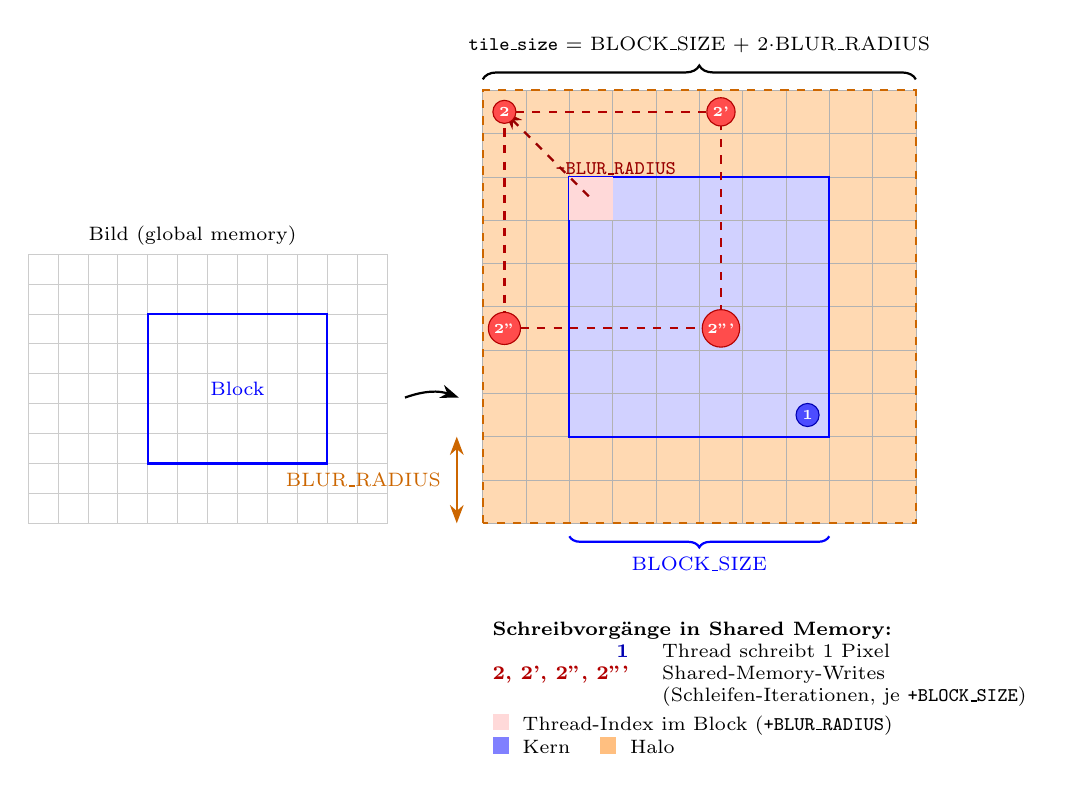
\begin{tikzpicture}[
        every node/.style={font=\scriptsize},
        >=Stealth
    ]

% ---------- LEFT: full image with tile position ----------
        \def\cellL{0.38cm}
        \begin{scope}[xshift=0cm]
            \foreach \x in {0,...,11}
            \foreach \y in {0,...,8}{
                \draw[gray!40, line width=0.2pt] (\x*\cellL, \y*\cellL) rectangle ++(\cellL,\cellL);
            }
            \draw[blue, thick] (4*\cellL, 2*\cellL) rectangle ++(6*\cellL, 5*\cellL);
            \node[align=center] at (5.5*\cellL, 9.6*\cellL) {Bild (global memory)};
            \node[blue, align=center] at (7*\cellL, 4.5*\cellL) {Block};
        \end{scope}

% ---------- connecting arrow ----------
        \draw[->, thick] (12.6*\cellL, 4.2*\cellL) to[out=20, in=160] (14.4*\cellL, 4.2*\cellL);

% ---------- RIGHT: zoomed tile with halo ----------
        \def\cellR{0.55cm}
        \def\radius{2}
        \def\blocksz{6}
        \begin{scope}[xshift=15.2*\cellL]

            % cells
            \foreach \x in {0,...,9}
            \foreach \y in {0,...,9}{
                \pgfmathtruncatemacro{\inCore}{(\x>=\radius) && (\x<\radius+\blocksz) && (\y>=\radius) && (\y<\radius+\blocksz)}
                \ifnum\inCore=1
                \fill[blue!18] (\x*\cellR, \y*\cellR) rectangle ++(\cellR,\cellR);
                \else
                    \fill[orange!30] (\x*\cellR, \y*\cellR) rectangle ++(\cellR,\cellR);
                \fi
            }
            \foreach \x in {0,...,10}
            \draw[gray!60, line width=0.2pt] (\x*\cellR, 0) -- (\x*\cellR, 10*\cellR);
            \foreach \y in {0,...,10}
            \draw[gray!60, line width=0.2pt] (0, \y*\cellR) -- (10*\cellR, \y*\cellR);

            \draw[blue, thick] (\radius*\cellR, \radius*\cellR) rectangle ++(\blocksz*\cellR, \blocksz*\cellR);
            \draw[orange!80!black, thick, dashed] (0,0) rectangle ++(10*\cellR, 10*\cellR);

            % marker (1): thread that writes exactly ONE pixel — moved clearly BELOW the
            % corner cluster now that the cluster sits at the top
            \node[circle, draw=blue!70!black, fill=blue!70!white, text=white, inner sep=1.2pt, font=\tiny\bfseries] (t1)
            at ({7.5*\cellR}, {2.5*\cellR}) {1};

            % marker (2, 2', 2'', 2'''): the corner thread (tx=0, ty=0) — full halo corner pixel.
            % Both i and j have TWO valid loop values (0 and BLOCK_SIZE), so this ONE thread
            % writes FOUR cells in total, forming a BLOCK_SIZE x BLOCK_SIZE square.
            \coordinate (cA) at ({0.5*\cellR}, {9.5*\cellR});                     % ORIGIN: i=tx, j=ty (Ecke oben links)
            \coordinate (cB) at ({(0.5+\blocksz-1)*\cellR}, {9.5*\cellR});         % i=tx+BLOCK_SIZE, j=ty (core) — 1 Zelle näher
            \coordinate (cC) at ({0.5*\cellR}, {(9.5-\blocksz+1)*\cellR});         % i=tx, j=ty+BLOCK_SIZE (core) — 1 Zelle näher
            \coordinate (cD) at ({(0.5+\blocksz-1)*\cellR}, {(9.5-\blocksz+1)*\cellR}); % beide +BLOCK_SIZE — 1 Zelle näher

            % the ACTUAL block-owned pixel of this same thread: (tx+radius, ty+radius) — always core,
            % highlighted light red and connected to the origin via the "-radius" shift
            \fill[red!15] ({\radius*\cellR}, {(9-\radius)*\cellR}) rectangle ++(\cellR,\cellR);
            \draw[<-, red!60!black, thick, dashed] (cA) -- ({(\radius+0.5)*\cellR}, {(9-\radius+0.5)*\cellR})
            node[midway, below right=-1pt] {\texttt{-BLUR\_RADIUS}};

            \draw[red!70!black, thick, dashed] (cA) rectangle (cD);

            \node[circle, draw=red!70!black, fill=red!70!white, text=white, inner sep=1.2pt, font=\tiny\bfseries] at (cA) {2};
            \node[circle, draw=red!70!black, fill=red!70!white, text=white, inner sep=1.2pt, font=\tiny\bfseries] at (cB) {2'};
            \node[circle, draw=red!70!black, fill=red!70!white, text=white, inner sep=1.2pt, font=\tiny\bfseries] at (cC) {2''};
            \node[circle, draw=red!70!black, fill=red!70!white, text=white, inner sep=1.2pt, font=\tiny\bfseries] at (cD) {2'''};

            % brace: tile_size (top)
            \draw[decorate, decoration={brace, amplitude=5pt}, thick]
            (0, {10.25*\cellR}) -- ({10*\cellR}, {10.25*\cellR})
            node[midway, above=6pt] {\texttt{tile\_size} = BLOCK\_SIZE + 2$\cdot$BLUR\_RADIUS};

            % brace: BLOCK_SIZE (below tile, own row so it never collides with legend)
            \draw[decorate, decoration={brace, amplitude=4pt, mirror}, thick, blue]
            ({\radius*\cellR}, {-0.3*\cellR}) -- ({(\radius+\blocksz)*\cellR}, {-0.3*\cellR})
            node[midway, below=4pt, blue] {BLOCK\_SIZE};

            % arrow: radius (halo thickness, left side)
            \draw[<->, orange!80!black, thick] (-0.6*\cellR, 0) -- (-0.6*\cellR, {\radius*\cellR})
            node[midway, left=2pt, align=center] {BLUR\_RADIUS};

            % ---- legend, well below everything else ----
            \node[align=left, anchor=north west] at (0, {-2.0*\cellR}) {
                \begin{tabular}{@{}rl@{}}
                    \multicolumn{2}{@{}l@{}}{\textbf{Schreibvorgänge in Shared Memory:}}\\
                    \textcolor{blue!70!black}{\textbf{1}} & Thread schreibt 1 Pixel\\
                    \textcolor{red!70!black}{\textbf{2, 2', 2'', 2'''}} & Shared-Memory-Writes\\
                    & (Schleifen-Iterationen, je \texttt{+BLOCK\_SIZE})\\[2pt]
                    \multicolumn{2}{@{}l@{}}{\textcolor{red!15}{\rule{6pt}{6pt}}\; Thread-Index im Block (\texttt{+BLUR\_RADIUS})}\\
                    \multicolumn{2}{@{}l@{}}{\textcolor{blue!50!white}{\rule{6pt}{6pt}}\; Kern \quad
                    \textcolor{orange!50!white}{\rule{6pt}{6pt}}\; Halo}
                \end{tabular}
            };

        \end{scope}

    \end{tikzpicture}
\end{document}